% book of game theory exercises
% nicola frosi
% starting date 05-06-2024

\documentclass[a4paper, twoside, openany]{book}

\usepackage[utf8]{inputenc}
\usepackage[T1]{fontenc}
\usepackage[english]{babel}

\usepackage[margin=2.5 cm]{geometry}

\usepackage{float}
\usepackage{rotating}


\usepackage{amsmath}
\usepackage{amsfonts}
\usepackage{amssymb}
\usepackage{amsthm}


\usepackage{enumitem}


\DeclareMathOperator*{\argmax}{arg\,max}
\DeclareMathOperator*{\argmin}{arg\,min}

\usepackage{tikz}
\usetikzlibrary{arrows.meta, calc, quotes}

\newcommand{\norm}[1]{\left\lVert#1\right\rVert}
\newcommand{\esssup}{\operatornamewithlimits{ess\,sup}}

\title{\textbf{\huge{\textit{A collection of Game Theory exercises}}}}

\begin{document}
\maketitle
\section*{Exercise $1$}
Two people are employed in a joint project. If every person $i=1,2$ spends an amount of resources $x_i$, where $0 \leq x_i \leq 1$, incurring a cost $k_i(x_i)$, the project will have a revenue of $f(x_1, x_2)$. The revenue is equally divided by the two persons, without considering the resources employed by each person.
\begin{itemize}
\item write the payoff function of each player;
\item formulate this problem as a strategic game and determine the possible Nash equilibria in the cases: 
				\begin{enumerate}
				\item $f(x_1, x_2) = 3 x_1 x_2 \qquad \textrm{and} \qquad k_i(x_i) = x_i^1 \qquad \textrm{for} \qquad i=1,2$;
				\item $f(x_1, x_2) = 4 x_1 x_2 \qquad \textrm{and} \qquad k_1(x_1) = x_1, \qquad k_2(x_2) = \frac{2}{3}x_2$.
				\end{enumerate}
\end{itemize}
In the prevoius cases can we deduce a priori that a Nash equilibrium exists?
\section*{Solution}
\textbf{case a)} \par
i) proceed:
$$f(x_1, x_2) = 3x_1 x_2,$$
the proceed for every single person is:
$$f_i(x_1, x_2) = \frac{3}{2} x_1 x_2.$$
The payoff functions are:
$$u_1(x_1, x_2) = \frac{3}{2}x_1 x_2 - x_1^2$$
$$u_2(x_1, x_2) = \frac{3}{2}x_1 x_2 - x_2^2.$$
The strategic game $(A_1 \times A_2, (u_1, u_2))$ is such that:
$$A_1 = A_2 = [0, 1]$$
$$u_1(x_1, x_2) = \frac{3}{2}x_1 x_2 - x_1^2$$
$$u_2(x_1, x_2) = \frac{3}{2}x_1 x_2 - x_2^2.$$
We now need to calculate the best reply:
$$BR_i:= A_{-i} \rightarrow A_i \qquad \forall i = 1, 2, \cdots, n,$$
that is
$$BR_1:= A_2 \rightarrow A_1 \qquad \forall x_2 \in [0, 1],$$
given by
$$BR_1(x_2) = \argmax_{x_1 \in [0,1]} u_1(x_1, x_2) = \argmax_{x_1 \in [0,1]} \frac{3}{2} x_1 x_2 - x_1^2 = \argmax_{x_1 \in [0, 1]} (\frac{3}{2}x_2 - x_1)x_1.$$
We have that
$$\frac{\partial u_1(x_1, x_2)}{\partial x_1} = \frac{3}{2}x_2 - 2 x_1 = 0$$
for
$$x_1 = \frac{3}{4}x_2,$$
so that
$$BR_1(x_2) = \frac{3}{4}x_2.$$
The best reply for the player two is:
$$BR_2:= A_1 \rightarrow A_2 \qquad \forall x_1 \in [0, 1]$$
given by
$$BR_1(x_1) = \argmax_{x_2 \in [0, 1]} u_2(x_1, x_2) = \argmax_{x_2 \in [0, 1]} \frac{3}{2}x_1 x_2 - x_2^2$$
so that
$$\frac{\partial u_2(x_1, x_2)}{\partial x_2} = \frac{3}{2}x_1 - x_2 = 0$$
for
$$x_2 = \frac{3}{4} x_1,$$
so that
$$BR_2(x_1) = \frac{3}{4}x_1.$$
\begin{figure}[!ht]
\begin{center}
\begin{tikzpicture}[scale=5.0]
\draw[->] (-0.2,0)--(1.5,0) node[below]{$x_1$};   
\draw[->] (0,-0.2)--(0,1.5)  node[left]{$x_2$};
\draw[dashed] (1.0,-0.2)--(1.0,1.2);
\draw[dashed] (-0.2,1.0)--(1.2,1.0);
\path
(0,0) node[below left]{$0$};
\path
(1.0,0) node[below right]{$1.0$};
\path
(0.0,1.0) node[below left]{$1.0$};
\foreach \i in {0,0.1, 0.2,...,1.0} \draw (\i,-0.02)--(\i,0.02);
\draw[green, domain=0.:1.0, samples=100, variable=\x] plot ({\x}, {3./4*\x});
\draw[orange, domain=0.:3./4, samples=100, variable=\x] plot ({\x}, {4./3*\x});
\path
(0.5,0.7) node[left]{$B_1$};
\path
(0.8,0.4) node[left]{$B_2$};
\filldraw [red] (0,0) circle (1pt) node[above left] (2.1) {$N.E.$};
\end{tikzpicture}
\end{center}
\end{figure}
We can also solve the following system:
$$\begin{cases}
	x_1 = \frac{3}{4}x_2 \\
	x_2 = \frac{3}{4}x_1
   \end{cases} \implies
   \begin{cases}
   x_1 = 0 \\
   x_2 = 0
   \end{cases}$$
$$(0,0) \qquad \textrm{is the unique Nash Equilibrium}.$$
\textbf{case b)} \par  
i) Payoff functions:
$$f(x_1, x_2) = 4 x_1 x_2,$$
then for each player the proceeds is
$$f_i(x_1, x_2) = 2x_1 x_2,$$
so that the payoff functions are:
$$u_1(x_1, x_2) = 2 x_1 x_2 - x_1$$
$$u_2(x_1, x_2) = 2x_1 x_2 - \frac{2}{3}x_1.$$
ii) Now we consider the two players strategic game $(A_1 \times A_2, (u_1, u_2))$ such that
$$A_1 = A_2 = [0, 1]$$
$$u_1(x_1, x_2) = 2 x_1 x_2 - x_1$$
$$u_2(x_1, x_2) = 2 x_1 x_2 - \frac{2}{3}x_2.$$
Now we can consider the Best Reply
$$BR_i:= A_{-i} \rightarrow A_i \qquad \forall i = 1, 2, \cdots, n$$
that are
$$BR_1:= A_2 \rightarrow A_1$$
$$BR_2:= A_1 \rightarrow A_2.$$ 
From the definition we have
$$BR_i(a_{-i}) = \{ a_i \in A_i \qquad \textrm{s.t.} \qquad u_i(a_{-i}, a_i) \geq u_i(a_{-i}, \hat{a}_i) \qquad \forall \hat{a}_i \in A_i \}$$
$$ = \argmax_{\hat{a}_i \in A_i} u_i(a_{-i}, \hat{a}_i)$$
$$BR_1(x_2) = \argmax_{x_1 \in [0,1]} (2x_1 - 1)x_1 = \begin{cases}
														\{ 0 \} \qquad \textrm{if} \qquad x_2 < \frac{1}{2} \\
														[0, 1] \qquad \textrm{if} \qquad x_2 = \frac{1}{2}\\
														\{ 1 \} \qquad \textrm{if} \qquad x_2 > \frac{1}{2}
													 \end{cases}$$
													 
\begin{figure}[!ht]
\begin{center}
\begin{tikzpicture}[scale=5.0]
\draw[->] (-0.2,0)--(1.5,0) node[below]{$x_1$};   
\draw[->] (0,-0.2)--(0,1.5)  node[left]{$x_2$};
\draw[dashed] (1.0,-0.2)--(1.0,1.2);
\draw[dashed] (-0.2,1.0)--(1.2,1.0);
\path
(0,0) node[below left]{$0$};
\path
(1.0,0) node[below right]{$1.0$};
\path
(0.0,1.0) node[below left]{$1.0$};
\foreach \i in {0,0.1, 0.2,...,1.0} \draw (\i,-0.02)--(\i,0.02);
\draw[blue, line width = 1.5] (0,0.0)--(0,0.5);
\draw[blue, line width = 1.5, domain=0.:1., samples=100, variable=\x] plot ({\x}, {0.5});
\draw[blue, line width = 1.5] (1.,0.5)--(1.,1.);
\path
(0.5,0.7) node[left]{$B_1$};
\end{tikzpicture}
\end{center}
\end{figure}			
$$BR_2 := A_1 \rightarrow A_2 \qquad \forall x_1 \in [0, 1]$$
$$BR_2(x_1) = \argmax_{x_2 \in [0, 1]} (2x_1 -\frac{2}{3})x_2 = \begin{cases}
																\{ 0 \} \qquad \textrm{if} \qquad x_1 < \frac{1}{3} \\
																[0, 1] \qquad \textrm{if} \qquad x_1 = \frac{1}{3}\\
																\{ 1 \} \qquad \textrm{if} \qquad x_1 > \frac{1}{3}
                                                                \end{cases}$$
                                   
\begin{figure}[!ht]
\begin{center}
\begin{tikzpicture}[scale=5.0]
\draw[->] (-0.2,0)--(1.5,0) node[below]{$x_1$};   
\draw[->] (0,-0.2)--(0,1.5)  node[left]{$x_2$};
\draw[dashed] (1.0,-0.2)--(1.0,1.2);
\draw[dashed] (-0.2,1.0)--(1.2,1.0);
\path
(0,0) node[below left]{$0$};
\path
(1.0,0) node[below right]{$1.0$};
\path
(0.0,1.0) node[below left]{$1.0$};
\foreach \i in {0,0.1, 0.2,...,1.0} \draw (\i,-0.02)--(\i,0.02);
\draw[green, line width = 1.5] (0,0.0)--(1./3,0.0);
\draw[green, line width = 1.5] (1./3,0.)--(1./3,1.);
\draw[green, line width = 1.5, domain=1./3:1., samples=100, variable=\x] plot ({\x}, {1.0});
\path
(0.5,0.7) node[left]{$B_2$};
\end{tikzpicture}
\end{center}
\end{figure}	
From the definition 
$$a^{\star} \in A \qquad \textrm{is a Nash Equilibrium}$$
$$\textrm{iff}$$
$$a_i^{\star} \in BR_i(a_{-i}^{\star} \qquad \forall i$$
\begin{figure}[!ht]
\begin{center}
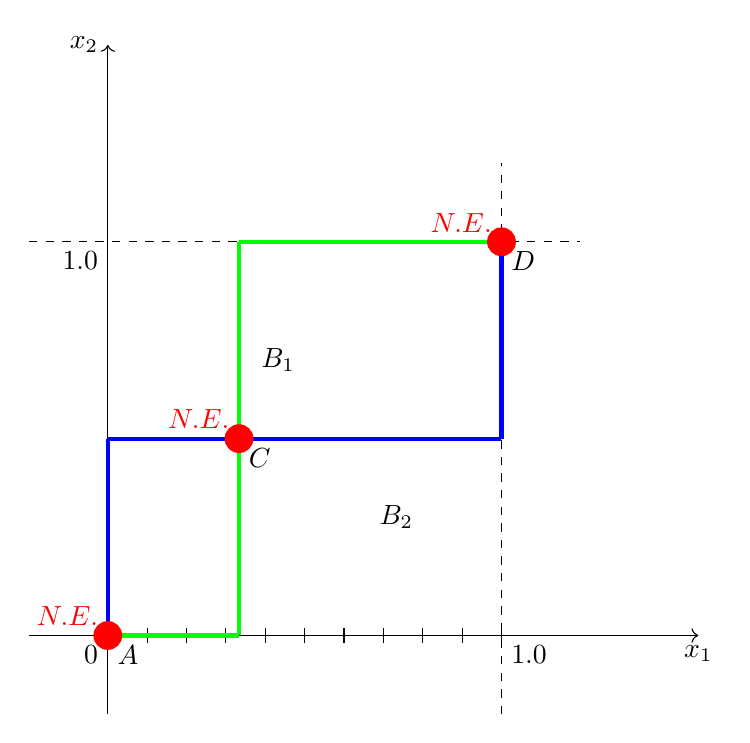
\begin{tikzpicture}[scale=5.0]
\draw[->] (-0.2,0)--(1.5,0) node[below]{$x_1$};   
\draw[->] (0,-0.2)--(0,1.5)  node[left]{$x_2$};
\draw[dashed] (1.0,-0.2)--(1.0,1.2);
\draw[dashed] (-0.2,1.0)--(1.2,1.0);
\path
(0,0) node[below left]{$0$};
\path
(1.0,0) node[below right]{$1.0$};
\path
(0.0,1.0) node[below left]{$1.0$};
\foreach \i in {0,0.1, 0.2,...,1.0} \draw (\i,-0.02)--(\i,0.02);
\draw[green, line width = 1.5] (0,0.0)--(1./3,0.0);
\draw[green, line width = 1.5] (1./3,0.)--(1./3,1.);
\draw[green, line width = 1.5, domain=1./3:1., samples=100, variable=\x] plot ({\x}, {1.0});
\draw[blue, line width = 1.5] (0,0.0)--(0,0.5);
\draw[blue, line width = 1.5, domain=0.:1., samples=100, variable=\x] plot ({\x}, {0.5});
\draw[blue, line width = 1.5] (1.,0.5)--(1.,1.);
\path
(0.5,0.7) node[left]{$B_1$};
\path
(0.8,0.3) node[left]{$B_2$};
\filldraw [red] (0,0) circle (1pt) node[above left] (2.1) {$N.E.$};
\filldraw [red] (1./3,1./2) circle (1pt) node[above left] (2.1) {$N.E.$};
\filldraw [red] (1.,1.) circle (1pt) node[above left] (2.1) {$N.E.$};
\path
(0.,0.) node[below right]{$A$};
\path
(1./3,1./2) node[below right]{$C$};
\path
(1.,1.) node[below right]{$D$};
\end{tikzpicture}
\end{center}
\end{figure}	
The Nash Equilibrium are
$$B_1 \cap B_2 = \{ A, C, D \}$$
where
$$A = (0,0)$$
$$C = (1./3, 1./2)$$
$$D = (1., 1.)$$
The functions $u_i: A_1 \times A_2 \rightarrow \mathbb{R}$ are continuous. The map $x_1 \mapsto u_1(x_1, x_2)$ with $x_2 \in A$ fixed is linear in $x_1$ and so it is concave. The same for the map $x_2 \mapsto u_2(x_1, x_2)$ with $x_1 \in A$ fixed. Then the Nash Theorem guarantees the existence of at least a Nash Equilibrium.
\clearpage
\section*{Exercise $2$}
Consider a two player non-cooperative game, in which every player controls a unique variable, which we indicate, respectively with $x_1$ for the first player and $x_2$ for the second player. The alternative set for the first player is:
$$X_1 = \{ x_1 \qquad \textrm{such that} \qquad -6 \leq x_1 \leq 2 \}$$
and for the second player is:
$$X_2 = \{ x_2 \qquad \textrm{such that} \qquad -2 \leq x_2 \leq 4 1 \}.$$
The payoff functions for the two players are:
$$C_1(x_1, x_2) = \frac{1}{2}x_1^2 - x_1(2x_2 - 4) + 7 x_2$$
$$C_2(x_1, x_2) = (3 - x_2)(1 - x_1).$$
\begin{enumerate}[label=\alph*.]
\item Can be stated "a priori" the existence of a Nash Equilibrium?
\item Identify for each player the Best Reply functions.
\item Identify the Nash Equilibrium of the game, if they exist. 
\end{enumerate}
\section*{Solution}
\textbf{Point a)} \par 
The two player strategic game is
$$(A_1 \times A_2, (u_1, u_2))$$
with the alternative sets:
$$A_1 = [-6, 2]$$
$$A_2 = [-2, 4],$$
and payoff functions
$$u_1(x_1, x_2) = \frac{1}{2}x_1^2 - x_1(2 x_2 - 4) + 7 x_2$$
$$u_2(x_1, x_2) = (3 - x_2)(1 - x_1),$$
where the two players must minimize. Now we verify the hypotheses of the Nash Theorem. \par 
$A_1$ and $A_2$ are closed and bounded sets of $\mathbb{R}$ so that they are non empty, convex and compact subsets of $\mathbb{R}$. The functions
$$u_i: A_1 \times A_2 \rightarrow \mathbb{R}$$
are continuous. The map
$$x_1 \mapsto u_1(x_1, x_2)$$
with $x_2 \in A_2$ fixed non-linear with respect to the variable $x_1$, but since we are considering a minimizing problem the map $x_1 \mapsto u_1(x_1, x_2)$ is convex for every $x_2$ fixed and so also for the map $x_2 \mapsto u_2(x_1, x_2)$ for every $x_1$ fixed. \par   
The hypotheses of the Nash Theorem are satisfied so we know that at least a Nash Equilibrium exists. \par  
\textbf{Point b)}
$$BR_i : A_{-i} \rightarrow A_i$$
$$BR_1 : A_2 \rightrightarrows A_1 \qquad \forall x_2 \in [-2, 4]$$
is given by
$$BR_1(x_2) = \argmin_{x_1 \in [-6, 2]} u_1(x_1, x_2) = \argmin_{x_1 \in [-6, 2]} \frac{1}{2}x_1^2 - x_1(2x_2 - 4) + 7 x_2$$
so that
$$\frac{\partial u_1(x_1, x_2)}{\partial x_1} = x_1 - (2 x_2 - 4) = 0$$
for
$$x_1 = 2 x_2 - 4.$$
\begin{figure}[!ht]
\begin{center}
\begin{tikzpicture}[scale=1.0]
\draw[->] (-7.2,0)--(5.5,0) node[below]{$x_1$};   
\draw[->] (0,-2.2)--(0,5.5)  node[left]{$x_2$};
\draw[dashed] (-6.0,-3.2)--(-6.0,3.2);
\draw[dashed] (2.0,-3.2)--(2.0,4.2);
\draw[dashed] (-6.0,-3.2)--(-6.0,4.2);
\draw[dashed] (-6.5,-2.0)--(2.5,-2.0);
\draw[dashed] (-6.5,4.0)--(2.5,4.0);
\path
(0,0) node[below left]{$0$};
\path
(-6.0,0) node[below right]{$-6.0$};
\path
(2.0,0) node[below right]{$2.0$};
\path
(0.0,1.0) node[below left]{$1.0$};
\path
(0.0,2.0) node[below left]{$2.0$};
\path
(0.0,3.0) node[below left]{$3.0$};
\path
(0.0,4.0) node[below left]{$4.0$};
\draw[red, line width = 2.5] (-6.0,-2.0)--(-6.0,-1.0);
\draw[red, line width = 2.5, domain=-6.:2., samples=100, variable=\x] plot ({\x}, {0.5*\x + 2});
\path
(-1.0,2.0) node[left]{$B_1$};
\end{tikzpicture}
\end{center}
\end{figure}	
$$BR_1(x_2) = \argmin_{x_1 \in [-6, 2]} u_1(x_1, x_2) = \begin{cases}
															\{ -6 \} \qquad \textrm{if} \qquad x_2 < -11 \\
															\{2 x_2 - 4 \} \qquad \textrm{if} \qquad -1 < x_2 < 3 \\
															\{ 2 \} \qquad \textrm{if} \qquad x_2 >3
															
													   \end{cases}$$
$$BR_2(x_1) = \argmin_{x_2 \in [-2, 4]} u_2(x_1, x_2) = \argmin_{x_2 \in [-2, 4]} (3 - x_2)(1 - x_1)$$
$$\frac{\partial u_2(x_1, x_2)}{\partial x_2} = x_1 - 1 = const. = \begin{cases}
																		\{ 4 \} \qquad \textrm{if} \qquad x_1 < 1 \\
																		\{ -2, 4 \} \qquad \textrm{if} \qquad x_1 = 1\\
																		\{ - 2 \} \qquad \textrm{if} \qquad x_1 > 1
																 \end{cases}$$
\begin{figure}[!ht]
\begin{center}
\begin{tikzpicture}[scale=1.0]
\draw[->] (-7.2,0)--(5.5,0) node[below]{$x_1$};   
\draw[->] (0,-2.2)--(0,5.5)  node[left]{$x_2$};
\draw[dashed] (-6.0,-3.2)--(-6.0,3.2);
\draw[dashed] (2.0,-3.2)--(2.0,4.2);
\draw[dashed] (-6.0,-3.2)--(-6.0,4.2);
\draw[dashed] (-6.5,-2.0)--(2.5,-2.0);
\draw[dashed] (-6.5,4.0)--(2.5,4.0);
\path
(0,0) node[below left]{$0$};
\path
(-6.0,0) node[below right]{$-6.0$};
\path
(2.0,0) node[below right]{$2.0$};
\path
(0.0,1.0) node[below left]{$1.0$};
\path
(0.0,2.0) node[below left]{$2.0$};
\path
(0.0,3.0) node[below left]{$3.0$};
\path
(0.0,4.0) node[below left]{$4.0$};
\draw[blue, line width = 2.5, domain=-6.:1., samples=100, variable=\x] plot ({\x}, {4.});
\draw[blue, line width = 2.5] (1.0,-2.0)--(1.0,4.0);
\draw[blue, line width = 2.5, domain=1.:2., samples=100, variable=\x] plot ({\x}, {-2.});
\path
(-1.0,2.0) node[left]{$B_2$};
\end{tikzpicture}
\end{center}
\end{figure}	
Now to determine the Nash Equilibrium we need to make the intersection $B_1 \cap B_2$.
\begin{figure}[!ht]
\begin{center}
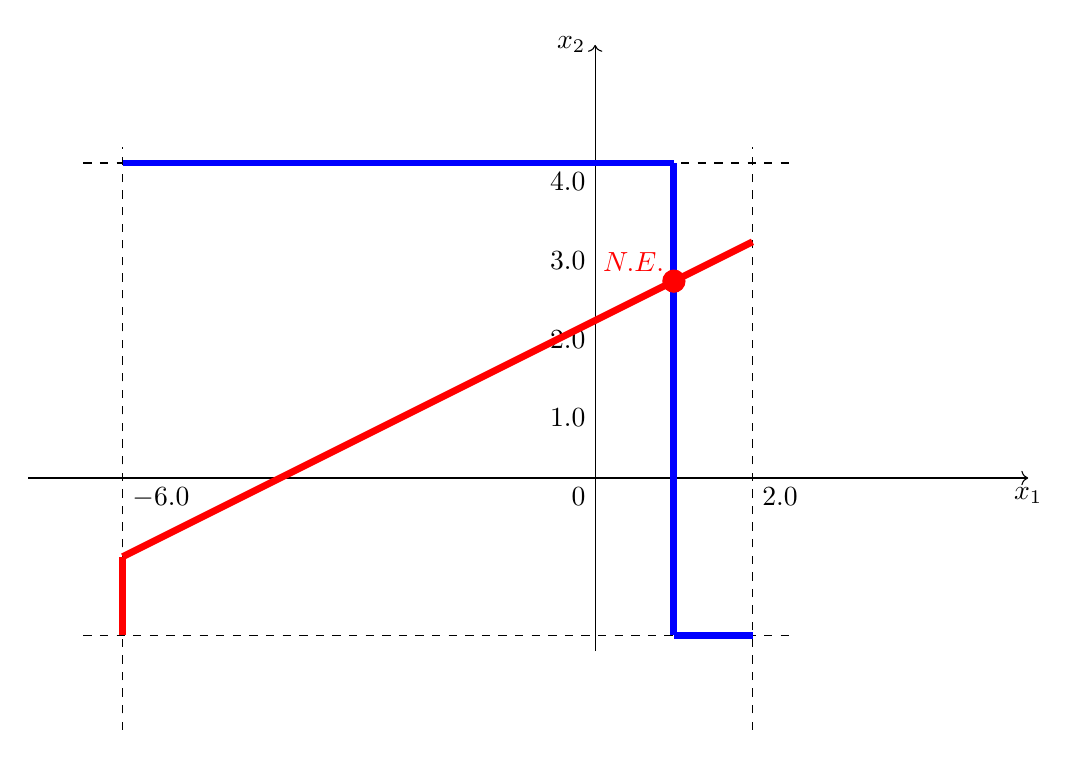
\begin{tikzpicture}[scale=1.0]
\draw[->] (-7.2,0)--(5.5,0) node[below]{$x_1$};   
\draw[->] (0,-2.2)--(0,5.5)  node[left]{$x_2$};
\draw[dashed] (-6.0,-3.2)--(-6.0,3.2);
\draw[dashed] (2.0,-3.2)--(2.0,4.2);
\draw[dashed] (-6.0,-3.2)--(-6.0,4.2);
\draw[dashed] (-6.5,-2.0)--(2.5,-2.0);
\draw[dashed] (-6.5,4.0)--(2.5,4.0);
\path
(0,0) node[below left]{$0$};
\path
(-6.0,0) node[below right]{$-6.0$};
\path
(2.0,0) node[below right]{$2.0$};
\path
(0.0,1.0) node[below left]{$1.0$};
\path
(0.0,2.0) node[below left]{$2.0$};
\path
(0.0,3.0) node[below left]{$3.0$};
\path
(0.0,4.0) node[below left]{$4.0$};
\draw[blue, line width = 2.5, domain=-6.:1., samples=100, variable=\x] plot ({\x}, {4.});
\draw[blue, line width = 2.5] (1.0,-2.0)--(1.0,4.0);
\draw[blue, line width = 2.5, domain=1.:2., samples=100, variable=\x] plot ({\x}, {-2.});
\draw[red, line width = 2.5] (-6.0,-2.0)--(-6.0,-1.0);
\draw[red, line width = 2.5, domain=-6.:2., samples=100, variable=\x] plot ({\x}, {0.5*\x + 2});
\filldraw [red] (1.,5./2) circle (4pt) node[above left] (2.1) {$N.E.$};
\end{tikzpicture}
\end{center}
\end{figure}	
We can also solve the following system:
$$\begin{cases}
		x_1 = 2 x_2 - 4 \\
		x_1 = 1
  \end{cases}$$
The the unique Nash Equilibrium is $(1; \frac{5}{2})$.
\clearpage
\section*{Exercise $3$}
Consider the following game:
\begin{center}
\begin{tabular}{|c | c | c| c| c| }
\hline
& Second Player & &  \\
\hline
 First Player & D & E & F\\
\hline
 A & $3 \qquad 0$ & $0 \qquad 0$ & $0 \qquad 3$ \\
\hline 
B & $0 \qquad 0$ &  $1 \qquad 1$ &  $0 \qquad 0$ \\
\hline  
C & $0 \qquad 3$ &  $0 \qquad 0$ &  $3 \qquad 0$ \\  
\hline 
\end{tabular}
\end{center}
\begin{enumerate}[label=\alph*.]
\item Determine the eventual Nash Equilibrium in pure strategy;
\item Show that there exists an Equilibrium in mixed strategies with the player $1$ that plays $(A, B, C)$ with probability $(\frac{1}{5}, \frac{3}{5}, \frac{1}{5})$ and the player $2$ that plays $(D, E, F)$ with probability $(\frac{1}{5}, \frac{3}{5}, \frac{1}{5})$.
\end{enumerate}
\section*{Solution}
\textbf{Point a)} \par 
\begin{itemize}
\item if player $2$ plays $D$ player $1$ to maximize chooses $A$;
\item if player $2$ plays $E$ player $1$ to maximize chooses $B$;
\item if player $2$ plays $F$ player $1$ to maximize chooses $C$;
\end{itemize}
\begin{itemize}
\item if player $1$ plays $A$ player $2$ to maximize chooses $F$;
\item if player $1$ plays $B$ player $2$ to maximize chooses $E$;
\item if player $1$ plays $C$ player $1$ to maximize chooses $D$;
\end{itemize}
Then the unique Nash Equilibrium in pure strategies is $(B, E)$.
\textbf{Point b)} \par  
$$A_1 = \{ A, B, C \}$$
$$A_2 = \{ D, E, F \}$$
$$S_i:= \Delta A_i$$
$$S_1 = \Delta A_1 = x_1 A + x_2 B + (1 - x_1 - x_2) C$$
with $x_1 + x_2 = 1 \qquad x_i \geq 0$.
$$S_2 = \Delta A_2 = y_1 D + y_2 E + (1 - y_1 - y_2) F$$
with $y_1 + y_2 = 1 \qquad y_i \geq 0$.
Now we can construct the payoff functions.
$$u_1(x_1, x_2, x_3, y_1, y_2, y_3) = [x_1, x_2, 1 - x_1 - x_2] \begin{bmatrix}
																	3 & 0 & 0 \\
																	0 & 1 & 0 \\
																	0 & 0 & 3 
                                                                \end{bmatrix} \begin{bmatrix}
                                                                y_1 \\
                                                                y_2 \\
                                                                1 - y_1 - y_2
                                                                \end{bmatrix}$$
$$= [3 x_1, x_2, 3(1 - x_1 - x_2)] \begin{bmatrix}
									y_1 \\
									y_2 \\
									1 - y_1 - y_2
								  \end{bmatrix} = 3 x_1 y_1 + y_2 x_2 + 3(1 - x_1 - x_2)(1 - y_1 - y_2)$$
$$= 3 x_1 y_1 + y_2 x_2 + 3( 1 - y_1 - y_2 - x_1 + x_1 y_1 + x_2 y_2 - x_2 + x_2 y_1 + x_2 y_2) $$
$$= 6 x_1 y_1 + 4x_2 y_2 + 3x_1 y_2 + 3x_2 y_1 - 3y_2 - 3x_1 - 3x_2 - 3y_1 + 3.$$
Thr payoff function for the second player:
$$u_2(x_1, x_2,x_3, y_1, y_2, y_3) = [x_1, x_2, 1 - x_1 - x_2] \begin{bmatrix}
																0 & 0 & 3\\
																0 & 1 & 0\\
																3 & 0 & 0
                                                               \end{bmatrix} \begin{bmatrix}
                                                               y_1 \\
                                                               y_2 \\
                                                               1 - y_1 - y_2
                                                               \end{bmatrix}$$
$$= [3(1 - x_1 - x_2), x_2, 3x_1]\begin{bmatrix}
									y_1 \\
									y_2 \\
									1 - y_1 - y_2
								\end{bmatrix} = 3y_1 - 6x_1y_1 + x_2 y_2 - 3x_2 y_1 -3x_1y_2 + 3x_1$$
Summarize:
$$u_1(x_1, x_2, y_1, y_2) = 6x_1 y_1 + 4x_2 y_2 + 3 x_1 y_2 + 3x_2 y_1 - 3y_2 - 3x_1 - 3x_2 - 3y_1 + 3$$
$$u_2(x_1, x_2, y_1, y_2) = -6 x_1 y_1 + x_2 y_2 - 3 x_2 y_1 - 3 x_1 y_2 + 3 y_1 + 3 x_1$$
$$BR_i : A_{-i} \rightrightarrows A_i$$
$$BR_1 : A_2 \rightrightarrows A_1.$$
In terms of a mixed strategic game $E(G)$, we have
$$BR_i : S_{-i} \rightrightarrows S_i$$
$$BR_1: S_2 \rightrightarrows S_1.$$
Now we fix $(y_1, y_2) \in [0, 1] \times [0, 1]$,
$$BR_1(y_1, y_2) = \argmax_{(x_1, x_2) \in [0,1]^2} u_1(x_1, x_2, y_1, y_2) = \argmax_{(x_1, x_2) \in [0, 1]^2} 6x_1y_1 + 4x_2y_2 + 3 x_1 y_2 + 3x_2 y_1 - 3 y_2 - 3x_1$$
$$= \argmax_{(x_1, x_2) \in [0, 1]^2} x_1(6 y_1 + 3 y_2 - 3) + x_2(4 y_2 + 3 y_1 -3).$$
$$BR_1(\frac{1}{5}, \frac{3}{5}, \frac{1}{5}) = \argmax_{(x_1, x_2) \in [0, 1]^2} x_1(\frac{6}{5} + \frac{9}{5} - \frac{15}{5}) + x_2(\frac{12}{5} + \frac{3}{5} - \frac{15}{5})= \argmax_{(x_1, x_2) \in [0, 1]^2} 0 = [0, 1] \times [0, 1].$$
$$S^{\star} = \bigl((\frac{1}{5}, \frac{3}{5}, \frac{1}{5}), (\frac{1}{5}, \frac{3}{5}, \frac{1}{5})\bigl)$$
$$S_1^{\star} = (\frac{1}{5}, \frac{3}{5}, \frac{1}{5})$$
$$BR_1^{\star}(S_2^{\star}) = x_1 A + x_2 D + (1 - x_1 - x_2) C$$
with $x_1, x_2 \in [0,1] \times [0,1]$. Considering
$$\frac{1}{5}A + \frac{3}{5}B + \frac{1}{5}C,$$
then we have verified that $S_1^{\star} \in BR_1(S_2^{\star})$.
$$BR_2 : S_1 \rightrightarrows S_2$$
we now fix $x_1, x_2 \in  [0,1] \times [0,1]$ so that
$$BR_2(x_1, x_2, 1- x_1 - x_2) = \argmax_{(y_1, y_2) \in [0,1]^2} u_2(x_1, x_2, y_1, y_2) = \argmax_{(y_1, y_2) \in [0, 1]^2} -6x_1 y_1 + x_2 y_2 -3 x_2 y_1 - 3x_1 y_2 + 3 y_1 + 3 x_1$$
$$= \argmax_{(y_1, y_2) \in [0, 1]^2} y_1(-6 x_1 - 3x_2 +3) + y_2(x_2 - 3x_1)$$
$$BR_2(\frac{1}{5}, \frac{3}{5}, \frac{1}{5}) = \argmax_{(y_1, y_2) \in [0,1]^2} y_1(-\frac{6}{5} - \frac{9}{5} + \frac{15}{5}) + y_2(\frac{3}{5} - \frac{3}{5}) = \argmax_{(y_1, y_2) \in [0,1]^2} 0 = [0,1] \times [0,1]$$
$$BR_2(S_1^{\star}) = [0, 1] \times [0, 1]$$
so that
$$BR_2^{\star}(S_1^{\star}) = y_1 D + y_2 E + (1 - y_1 - y_2)F$$
with $(y_1, y_2) \in [0, 1]^2$. Since
$$S_2^{\star} = (\frac{1}{5}, \frac{3}{5}, \frac{1}{5}),$$
we have
$$\frac{1}{5}D + \frac{3}{5}E + \frac{1}{5}F$$
then $S_2^{\star} \in BR_2(S_1^{\star})$. \par   
Since
$$S_1^{\star} \in BR_1(S_2^{\star})$$
and
$$S_2^{\star} \in BR_2(S_1^{\star})$$
there exists a Nash Equilibrium in mixed strategies with the player $1$ that plyas 
$$\frac{1}{5}A + \frac{3}{5}B + \frac{1}{5}C$$
and the player $2$ that plays
$$\frac{1}{5}D + \frac{3}{5}E + \frac{1}{5}F.$$
\end{document}